\section{Examples}
We provide examples of some of the LaTeX features and packages we use most.
This is both a visual check that our template formats things the way we
want to, and a reference on how to use relevant LaTeX features.

\subsection{Citation}
We use \lstinline{BibLaTeX} \cite{biblatex} for bibliography management . The
bibliography will automatically only include the references which were cited in
the document.

Citations look like:
\begin{itemize}
\item Single citation: \cite{Gehrels:2016}.
\item Two citations: \cite{inkscape,gnuplot}.
\item Citations list: \cite{inkscape,gnuplot,thomashoullier/alarm-clock}
\end{itemize}

\subsection{Acronyms}
We use \lstinline{glossaries} \cite{glossaries} for acronyms list and eventual
glossaries (not included in the present template).  Acronyms are defined in a
list at the beginning of the document. Only actually used acronyms are
included. The acronyms are defined in the text automatically the first time
they are used.

For instance:
\begin{itemize}
\item First use: \gls{RBF}.
\item Subsequent uses: \gls{RBF}.
\end{itemize}

\subsection{Equations}
Equations are written in the usual manner (see
\cref{eq:example,eq:example2,eq:example3}).

\begin{equation} \label{eq:example}
\int_{a}^{b} \omega(x) f(x) \approx \sum_{i=1}^n w_i f(x_i)
\end{equation}

\begin{equation} \label{eq:example2}
\begin{cases}
p_{n+1}(x) = (A_n x + B_n) p_n(x) - C_n p_{n-1}(x) \\
p_0(x) = 1 \\
p_1(x) = A_0 x + B_0
\end{cases}
\end{equation}

\begin{equation} \label{eq:example3}
e^{ - at} \cos (\Omega t)u(t) \Leftrightarrow
\frac{{s + a}}{{(s + a)^2  + \Omega ^2 }}
\end{equation}

See the LaTeX equation examples at \cite{equationsheet,SO-latex-equations}.

\subsection{Figures}
Figures have the following appearance (see \cref{fig:svg,fig:sinus,fig:photo}).
We use the package \lstinline{svg} \cite{svg} for importing \gls{svg} files.

\begin{figure}
\includesvg[width=.6\textwidth]{images/inkscape-logo.svg}
\caption{\label{fig:svg} Example vector image in svg format. This is the
Inkscape™ logo. Inkscape is a \gls{svg} editor \cite{inkscape}.}
\end{figure}

\begin{figure}
\includesvg[width=.7\textwidth]{images/gp-sin/sinus.svg}
\caption{\label{fig:sinus} Example plot in svg format. Created using gnuplot
\cite{gnuplot}.}
\end{figure}

\begin{figure}
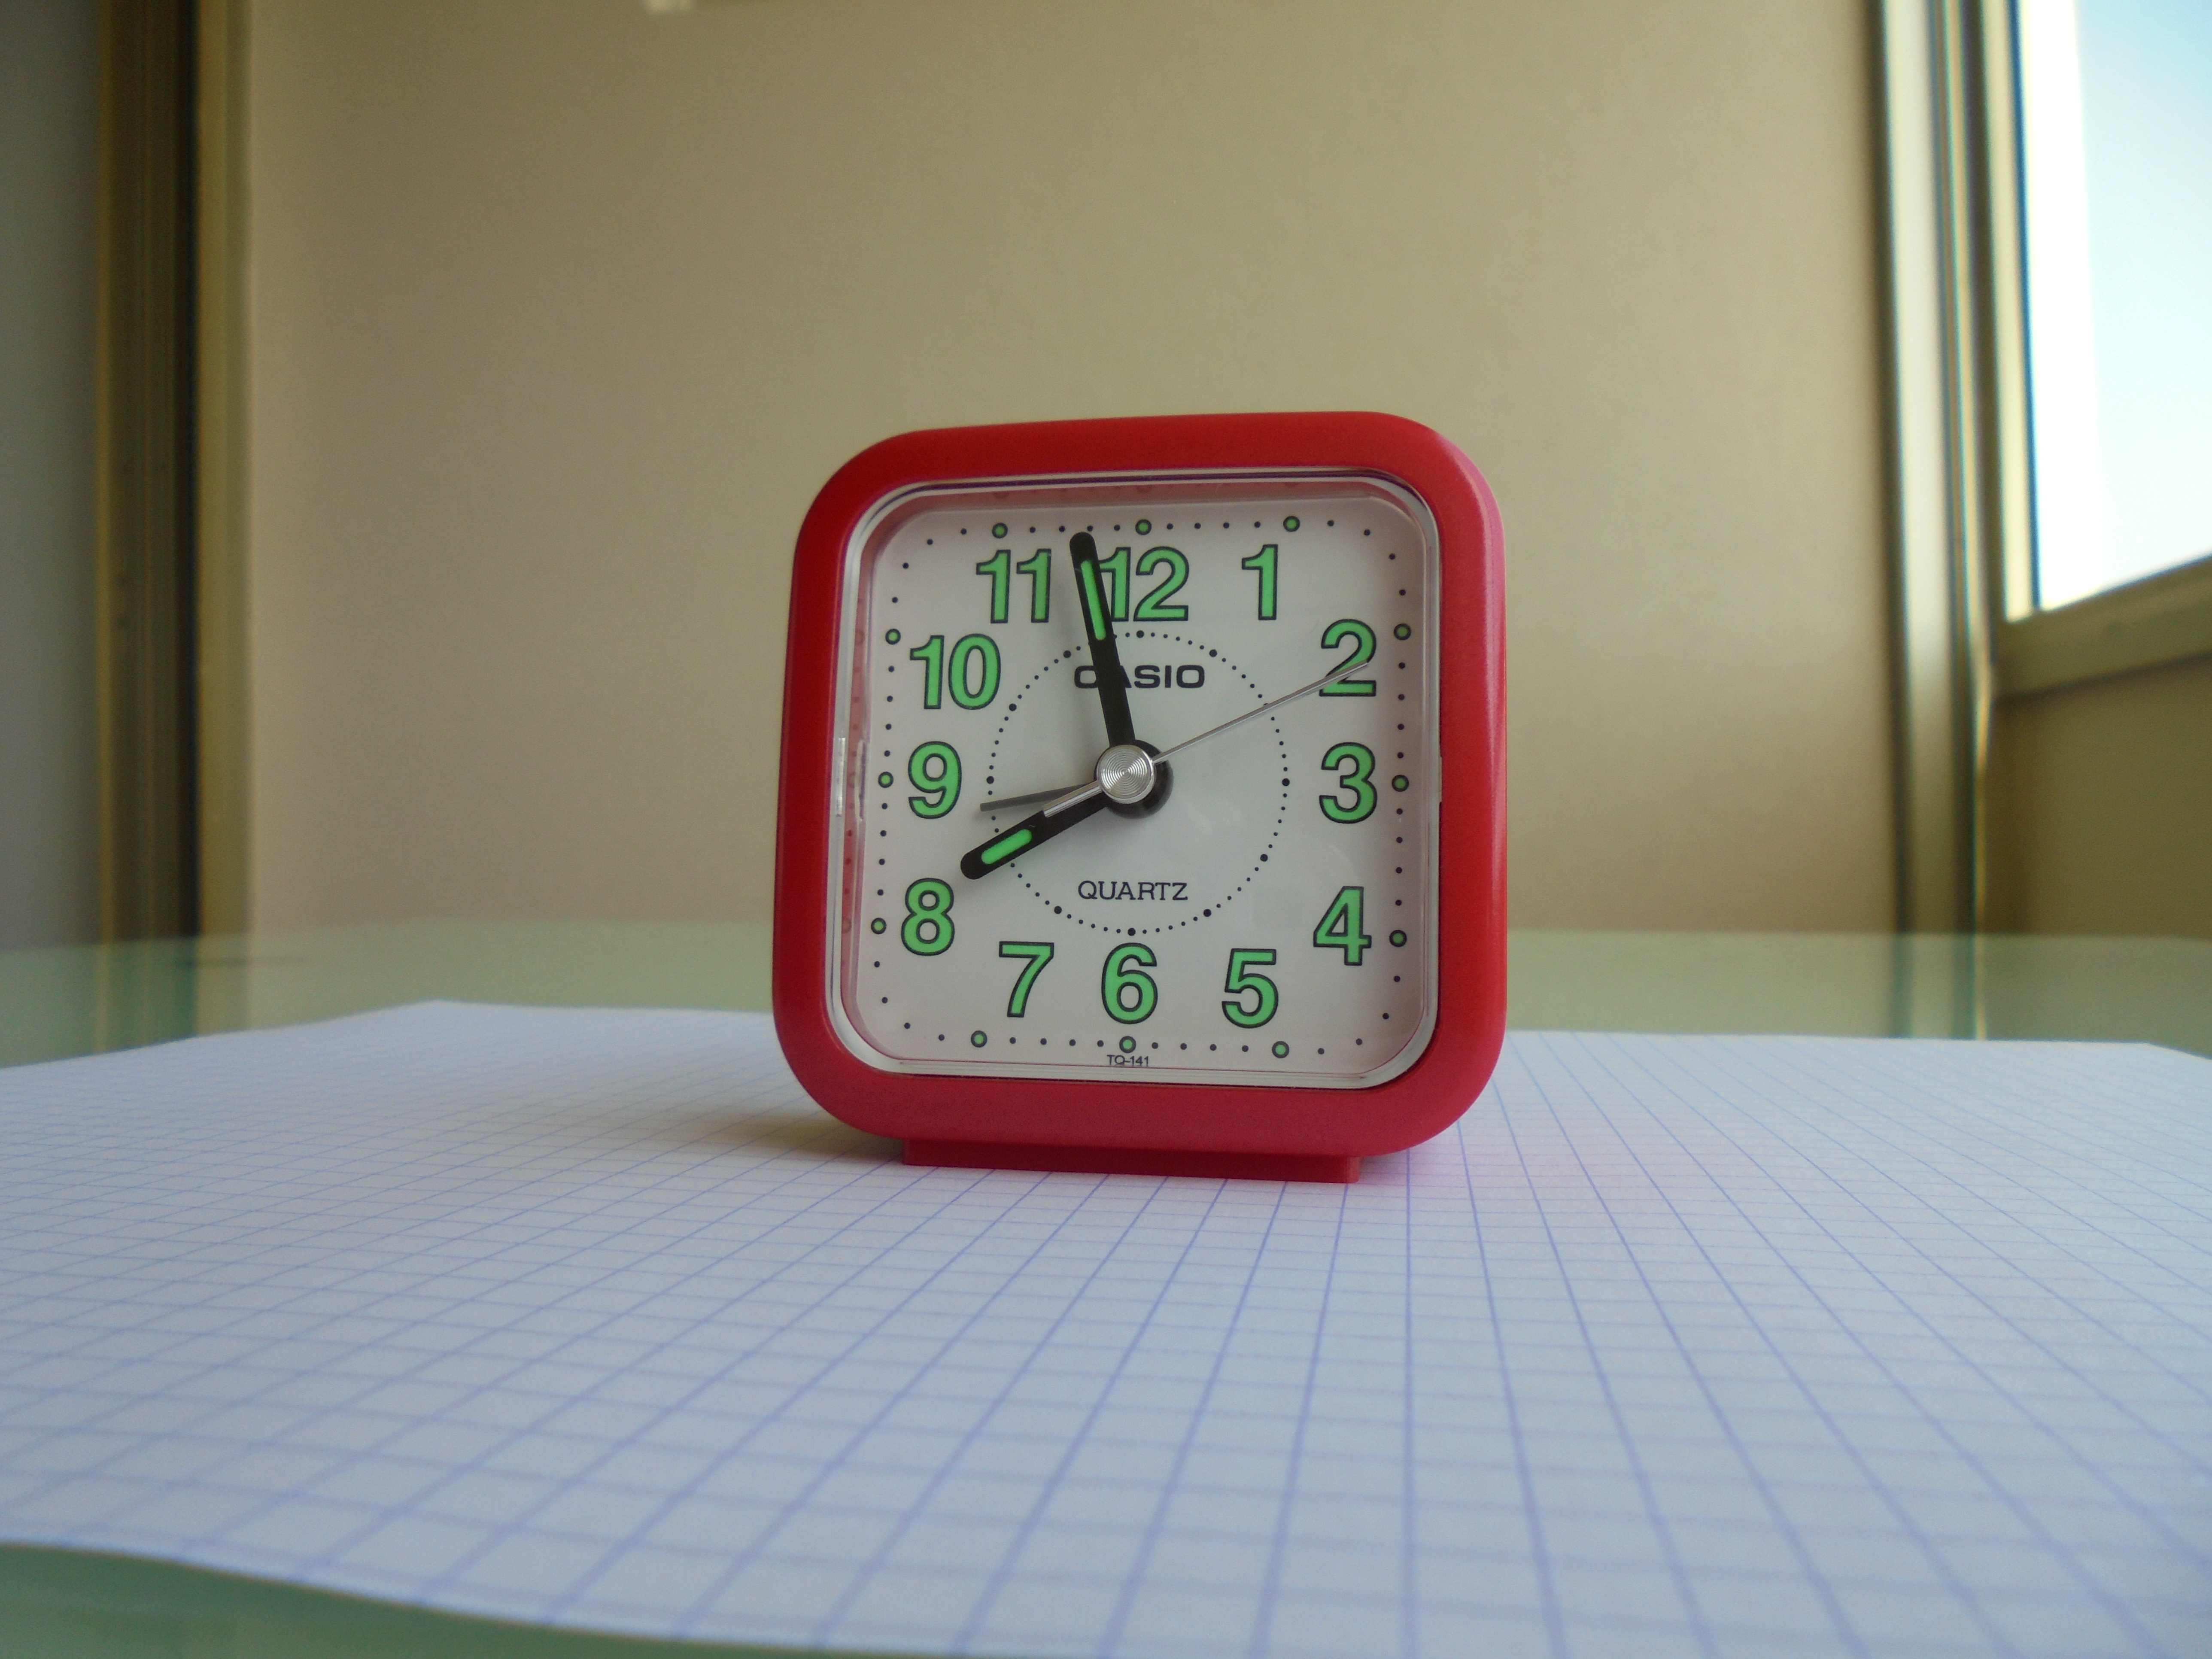
\includegraphics[width=\textwidth]{images/photo-alarm-clock.jpg}
\caption{\label{fig:photo} Example raster image: photograph from
\cite{thomashoullier/alarm-clock}.}
\end{figure}

My own rules of thumb regarding the format of images are:
\begin{itemize}
\item \textbf{Vector images}, such as \gls{svg}: I use \gls{svg} as much
as possible. I find this important with respect to the feeling of quality
a document inspires. I make an exception for images with a number of elements
that would be excessive for document rendering.
\begin{itemize}
\item Diagrams: can be edited with Inkscape \cite{inkscape}.
\item Plots: can be generated by gnuplot \cite{gnuplot}.
\item Logos: Most logos have a vector version.
\end{itemize}
\item \textbf{Raster images}
\begin{itemize}
\item Photographs: Raster representations are well suited to photographs.
      Most photographs should be compressed, depending on what the author
      wants to show, so as not to add unnecessary weight to the output document.
      The tool jpegoptim \cite{tjko/jpegoptim} is well suited for this purpose.
      I find both \gls{jpg} and WEBP formats to give good results.
\item Screenshots: Screenshots generally contain large areas filled with a
      single color. \gls{png} and WEBP are recommended here.
\end{itemize}
\end{itemize}

\subsection{Tables}
Tables may be created in the usual way (see
\cref{tab:example1,tab:example2,tab:example3}).

\begin{table} \caption{\label{tab:example1} Example table.}
\begin{tabular}{l | c c c} \hline
1 & a & b & c \\ \hline
2 & d & e & f \\ \hline
3 & g & h & i \\
\hline \end{tabular}
\end{table}

\begin{table} \caption{\label{tab:example2} Example table: second.}
\begin{tabular}{l | c c c} \hline
4 & j & k & l \\ \hline
5 & m & n & o \\ \hline
6 & p & q & r \\
\hline \end{tabular}
\end{table}

\begin{table} \caption{\label{tab:example3} Example table: third.}
\begin{tabular}{l | c c c} \hline
7 & s & t & u \\ \hline
8 & v & w & x \\ \hline
9 & y & z & $\chi$ \\
\hline \end{tabular}
\end{table}

\subsection{Algorithms}
Algorithms use the \lstinline{algorithm2e} \cite{algorithm2e} package.
Algorithms may be typeset as follows
(see \cref{alg:euclid-gcd,alg:eratosthenes-sieve,alg:disjoint-decomp}).

\begin{algorithm}
\caption{\label{alg:euclid-gcd} Euclid's algorithm for \gls{GCD}
\cite{enwiki:euclid-algorithm}.}

\Input{$(A, B) \in \mathbb{N}$}
\KwResult{$\text{gcd}(A, B)$}
\BlankLine
$X \gets A$\;
$Y \gets B$\;
\While{$X \neq Y$}{
  \eIf{$X > Y$}
    {$X \gets X - Y$}
    {$Y \gets Y - X$}}
\KwRet{$X$}
\end{algorithm}

\begin{algorithm}
\caption{\label{alg:eratosthenes-sieve} Eratosthenes' Sieve
         \cite{enwiki:eratosthenes-sieve}.}
\Input{$n \in \mathbb{N}, n>1$}
\KwResult{Set of prime numbers from $2$ up to $n$}
$A \gets$ array of boolean elements set to True, indexed from $2$ up to $n$.\;
\For{$i \in \llbracket 2, \floor{\sqrt(n)} \rrbracket$}{
  \If{A[i]}{
    \For{$j \in \llbracket 0, \floor{\frac{n - i^2}{i}} \rrbracket$}{
      A[i] $\gets$ False\;
    }}}
\KwRet{Every i such that A[i]}
\end{algorithm}

\begin{algorithm}
\caption{\label{alg:disjoint-decomp} Disjoint Decomposition
         (sample in \cite{algorithm2e}).}
\SetKwData{Left}{left}\SetKwData{This}{this}\SetKwData{Up}{up}
\SetKwFunction{Union}{Union}\SetKwFunction{FindCompress}{FindCompress}
\Input{A bitmap $Im$ of size $w\times l$}
\Output{A partition of the bitmap}
\BlankLine
\emph{special treatment of the first line}\;
\For{$i\leftarrow 2$ \KwTo $l$}{
\emph{special treatment of the first element of line $i$}\;
\For{$j\leftarrow 2$ \KwTo $w$}{\label{forins}
\Left$\leftarrow$ \FindCompress{$Im[i,j-1]$}\;
\Up$\leftarrow$ \FindCompress{$Im[i-1,]$}\;
\This$\leftarrow$ \FindCompress{$Im[i,j]$}\;
\If(\tcp*[h]{O(\Left,\This)==1}){\Left compatible with \This}{\label{lt}
\lIf{\Left $<$ \This}{\Union{\Left,\This}}
\lElse{\Union{\This,\Left}}
}
\If(\tcp*[f]{O(\Up,\This)==1}){\Up compatible with \This}{\label{ut}
\lIf{\Up $<$ \This}{\Union{\Up,\This}}
\tcp{\This is put under \Up to keep tree as flat as possible}\label{cmt}
\lElse{\Union{\This,\Up}}\tcp*[h]{\This linked to \Up}\label{lelse}
}
}
\lForEach{element $e$ of the line $i$}{\FindCompress{p}}
}
\end{algorithm}

\subsection{Inline code and Blocks of code}
The package \lstinline{listings} \cite{listings} is used to display inline
code, verbatim characters and sentences, and blocks of code. It features
automatic syntax highlighting for most common programming languages.  Commands
can be inlined: \lstinline[style=mystyle,language=sh]{cat /etc/group}.  Blocks
of code are written as \cref{lst:python,lst:octave,lst:common-lisp}.

\begin{minipage}{\linewidth}
\begin{lstlisting}[language=Python,
                   caption={Python code sample \cite{numpy-hfft}.},
                   label={lst:python}]
>>> signal = np.array([1, 2, 3, 4, 3, 2])
>>> np.fft.fft(signal)
array([15.+0.j,  -4.+0.j,   0.+0.j,  -1.-0.j,   0.+0.j,  -4.+0.j]) # may vary

>>> np.fft.hfft(signal[:4]) # Input first half of signal
array([15.,  -4.,   0.,  -1.,   0.,  -4.])

>>> np.fft.hfft(signal, 6)  # Input entire signal and truncate
array([15.,  -4.,   0.,  -1.,   0.,  -4.])
\end{lstlisting} \end{minipage}

\begin{minipage}{\linewidth}
\begin{lstlisting}[language=Octave,
                   caption={Octave code sample \cite{octave-example}.},
                   label={lst:octave}]
m = rows (A); n = columns (A);
[U, S, V] = svd (A);
## determine the regularization factor alpha
## alpha =
## transform to orthogonal basis
b = U'*b;
## Use the standard formula, replacing A with S.
## S is diagonal, so the following will be very fast and accurate.
x = (S'*S + alpha^2 * eye (n)) \ (S' * b);
## transform to solution basis
x = V*x;
\end{lstlisting} \end{minipage}

\begin{minipage}{\linewidth}
\begin{lstlisting}[language=Lisp,
                   caption={Common Lisp code sample
                            \cite{common-lisp-example}.},
                   label={lst:common-lisp}]
(defun entropy (string &aux (length (length string)))
  (declare (type string string))
  (let ((table (make-hash-table)))
    (loop for char across string
          do (incf (gethash char table 0)))
    (- (loop for freq being each hash-value in table
             for freq/length = (/ freq length)
             sum (* freq/length (log freq/length 2))))))
\end{lstlisting} \end{minipage}

\subsection{Footnotes}
Footnotes may be included with the native feature \footnote{Hello}.

\subsection{Epigraphs}
\epigraph{Respondeo dicendum quod necesse est dicere spiritum sanctum a filio
esse. Si enim non esset ab eo, nullo modo posset ab eo personaliter distingui.}
{Sanctus Thomas Aquinas -- Summa Theologiae I, q.36, a.2}

Epigraphs can be included thanks to \lstinline{epigraph} \cite{epigraph}.
They are meant for the beginning of sections in this template.

\subsection{Icons}
The \lstinline{fontawesome} package \cite{fontawesome-latex} may be used for
small icons in-line with the text \faSmileO~\faMedkit~\faBicycle.

\subsection{Cross-references}
We use \lstinline{cleveref} \cite{cleveref} for cross-referencing.  We list
cases of cross-referencing to check how they look.

\begin{itemize}
\item Equations
\begin{itemize}
  \item Single: \cref{eq:example}.
  \item Two: \cref{eq:example,eq:example2}.
  \item List: \cref{eq:example,eq:example2,eq:example3}.
\end{itemize}
\item Figures
\begin{itemize}
  \item Single: \cref{fig:svg}.
  \item Two: \cref{fig:svg,fig:sinus}.
  \item List: \cref{fig:svg,fig:sinus,fig:photo}
\end{itemize}
\item Tables
\begin{itemize}
  \item Single: \cref{tab:example1}.
  \item Two: \cref{tab:example1,tab:example2}.
  \item List: \cref{tab:example1,tab:example2,tab:example3}.
\end{itemize}
\item Algorithms
\begin{itemize}
  \item Single: \cref{alg:euclid-gcd}
  \item Two: \cref{alg:eratosthenes-sieve,alg:euclid-gcd}
  \item List: \cref{alg:eratosthenes-sieve,alg:euclid-gcd,alg:disjoint-decomp}
\end{itemize}
\item Listings
\begin{itemize}
  \item Single: \cref{lst:python}
  \item Two: \cref{lst:octave,lst:python}
  \item List: \cref{lst:octave,lst:python,lst:common-lisp}
\end{itemize} \end{itemize}

\subsection{Revision history}
The revision history at the beginning of this document is created using
\lstinline{vhistory} \cite{vhistory}.
